\documentclass{article}
\usepackage{exercise}
\usepackage[obeyspaces]{url}
\usepackage[dvipsnames]{xcolor}
\usepackage{graphicx}
\usepackage{listings}
\usepackage[scaled]{helvet}
\usepackage{amsmath,amssymb,amsfonts,mathtools,cancel}

% typeset in helvetica
\renewcommand*\familydefault{\sfdefault} 

\newcommand{\ipi}{i-PI}
\newcommand{\hints}[1]{\emph{Hints: #1}}
\newcommand{\lstinxml}{\lstinline[language=XML]}
\newcommand{\lstinbash}{\lstinline[language=Bash]}
\usepackage[space=true]{accsupp}

\newcommand{\pdfactualhex}[3]{\newcommand{#1}{%
\BeginAccSupp{method=hex,ActualText=#2}#3\EndAccSupp{}}}

% PASTABLE lstlisting code
\pdfactualhex{\pdfactualdspace}{2020}{\textperiodcentered\textperiodcentered}
\pdfactualhex{\pdfactualsquote}{27}{'}
\pdfactualhex{\pdfactualbtick}{60}{`}

\lstset{tabsize=4,basicstyle=\ttfamily,breaklines=true,columns=flexible,emptylines=10000}
\lstset{literate={'}{\pdfactualsquote}1
                 {`}{\pdfactualbtick}1
                 {\ \ }{\pdfactualdspace}2
}

\lstset{
    basicstyle=\ttfamily,
    keywordstyle=\color{BrickRed},
    commentstyle=\color{Gray},
    stringstyle=\color{black},
    emphstyle=\color{RedOrange},
    columns=flexible,
    showstringspaces=false,
    xleftmargin=1em,
    deletekeywords={bin,all}
}


\lstdefinelanguage{Bash}
{
   alsodigit={-,.},
   morekeywords={ cp2k.popt, lmp_ubuntu, i-pi, vmd, for, done, python, mpirun, touch, tail, trajworks, autocorr, awk, i-pi-mergebeadspdb, grep, head, cp, cd, cat, ls, pwd, bash, sed, mkdir, vi, sh}
   %morecomment=[s][\color{orange}]{#}{\}
}

%\lstdefinelanguage{Python}
%{
%    morecomment=[s][\color{orange}]{#}{\}
%}


\lstdefinelanguage{XML}
{
  morestring=[b][\color{RedOrange}]",
%  morestring=[s]{>}{<},
  morecomment=[s]{<?}{?>},
  morecomment=[s][\color{orange}]{<!--}{-->},
  identifierstyle=\color{BlueViolet},
  keywordstyle=\color{ForestGreen},
  stringstyle=\color{RedOrange},
%  tagstyle=\color{Blue},
  morekeywords={xmlns,version,type, mode, units, forcefield, filename, stride, overwrite, nbeads,prefix}% list your attributes here
}

\lstdefinestyle{XML}
{
\tagstyle=\color{Blue}
}

\title{Introduction path integral \\molecular dynamics using \ipi{}}
\author{Venkat Kapil, Bingqing Cheng}
\date{June 2016}

\begin{document}

\maketitle

% INTRO
In this set of exercises we will learn 
about the basics of doing path integral 
molecular dynamics simulations using \ipi{}. 
We will begin by performing conventional
molecular dynamics simulation of classical nuclei,
and move towards highly quantum mechanical systems.
During the process, the design principles, 
features and input/output format of \ipi{} 
will be introduced.

\begin{Exercise}[label={basic},title={Molecular Dynamics simulations doing in a different way:  server and clients}]

What are the basic elements of Molecular Dynamics? 
Under the Born-Oppenheimer
approximation, the dynamics of the electronic
degrees of freedom is completely decoupled from that of the nuclei, and the electrons always
occupy the ground state for each configuration of the nuclei. 
In a fully classical treatment of nuclei, the
additional assumption is made that their 
dynamics can be described in terms of the 
Hamiltonian
\begin{equation}
    H(\textbf{p},\textbf{q})=\sum_i \dfrac{\textbf{p}_i^2}{2 m_i} + V(\textbf{q}),
\end{equation}
where $m_i$, $\textbf{p}_i$ and $\textbf{q}_i$ 
are the mass, the momentum and the coordinates of the $i$-th nucleus, respectively.

How shall we translate this Hamiltonian into a 
piece of computer program that automatically 
propagates the dynamics?
At first the equation of motion can be written as
\begin{equation}
   \dfrac{d \textbf{p}}{d t}= 
   \dfrac{\partial H(\textbf{p},\textbf{q})}{\partial \textbf{q}},
   ~\dfrac{d \textbf{q}}{d t}= 
   -\dfrac{\partial H(\textbf{p},\textbf{q})}{\partial \textbf{p}}.
\end{equation}
And then the time domain can be discretized into small  and finite time steps with length $\Delta t$.
The key processes are illustrated in this flow chart.
\begin{figure}
    \centering
    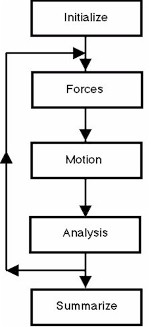
\includegraphics[width=0.25\textwidth]{mdchart.jpg}
\end{figure}
At the initialization stage, the program is informed about some basic information about the system,
such as the number of atoms, their types, system size, etc.
After that, the program goes through the loop ``Forces $\rightarrow$ Motion $\rightarrow$ Analysis" once per discrete simulation time step.
The force acting on each atom $\textbf{f}_i=\dfrac{\partial V}{\partial \textbf{q}_i}$ is evaluated first,
and are then used to advance the momenta and the coordinates of the nucleus such as
$\textbf{p}_i(t+\Delta t)\leftarrow \textbf{p}_i(t)+\textbf{f}_i \Delta t$ and 
$\textbf{q}_i(t+\Delta t)\leftarrow \textbf{q}_i(t)+\dfrac{\textbf{p}_i}{m_i} \Delta t$, 
 in its simplest form.
At the analysis step, the properties of interest for the system can be computed, stored, or analyzed on the fly.

From the flow chart of Molecular Dynamics, one can observe that each block of the program can be easily modularized.
One can even carry out the force evaluation using one piece of code,
communicate the results to another program, which does the motion and the analysis parts.
This is precisely the philosophy behind i-PI,
which acts like a server that takes care of the evolution of nuclei and the evaluation of
properties of the system.
And client codes evaluates forces and potential energy, and forward them to \ipi{}.

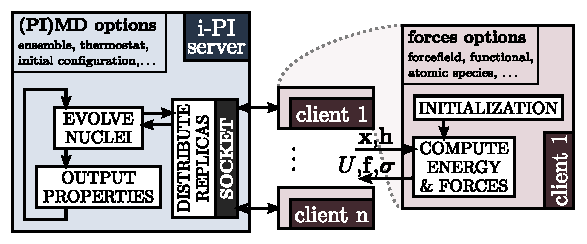
\includegraphics[width=1.0\textwidth]{ipi-scheme.pdf}

In this exercise, we will perform a simple Molecular Dynamics (MD) calculation.
Instead of doing the simulation directly using out-of-the-box MD software such as LAMMPS,
we are going to complete the task in a slightly more complex way.
We are going to use i-PI in conjunction with LAMMPS to demonstrate the work principles of i-PI 
as well as the subtle advantages that it brings.
The simulation will be performed on one gas phase water molecule using NVT ensemble at 300K.
We will also record the kinetic and potential energy of the system.

\Question
Read the LAMMPS input file \url{ex-1/300K-G-h2o/in.water}.
The force field specifications
\begin{lstlisting}[language=bash]
pair_style lj/cut/tip4p/long 1 2 1 1 0.278072379 17.007
bond_style class2 
angle_style harmonic
kspace_style pppm/tip4p 0.0001
\end{lstlisting}
means that a q-TIP4P force field is being used~\cite{habe-mano11pccp}.

On the parts of the input file that specifies how motions are propagated,
this line
\begin{lstlisting}[language=bash]
fix 1 all ipi 300K-G.0 32345 unix
\end{lstlisting}
is used, which basically means LAMMPS will only be in charge of the force evaluation and send that information to \ipi{}.
The latter will take care of the motion and the analysis parts.
All the information will be transmitted through a UNIX-domain socket with the name \url{300K-G.0},
which is a mechanism for local, inter-process communication.

\Question
Now open the \ipi{} input file \url{input.xml} in the same folder.
For a moment let us ignore all the other entries but only focus on the followings
\begin{lstlisting}[language=xml]
 <ffsocket name="tip4p" pbc="true" mode="unix">
    <address> 300K-G.0 </address>
 </ffsocket>
\end{lstlisting}
This indicates that \ipi{} will receive any information sent by LAMMPS through the UNIX-domain socket with the tag \url{300K-G.0},
and send the coordinates of the nuclei in the system to LAMMPS for force evaluations using the same socket.

\Question
Let's run an \ipi{}+LAMMPS Molecular Dynamics simulation!
Open a terminal at the current directory and
launch \ipi{} by typing
\begin{lstlisting}[language=bash]
$ i-pi input.xml
\end{lstlisting}
At this point \ipi{} should start 
%and show a logo like this
%\begin{figure}[h]
%\centering
%    
\includegraphics[width=0.2\textwidth]{ipi-logo.pdf}
%\end{figure}
and parse the input file. At the bottom of the output on the screen it should say
\begin{lstlisting}[language=bash]
Created unix socket with address 300K-G.0
@ForceField: Starting the polling thread main loop.
\end{lstlisting}
This means \ipi{} has started properly, has created the UNIX socket, and is waiting for the communications from the clients that do force evaluations.

\Question
Now it is a good time to start LAMMPS.
Open up a second terminal either manually or by typing \url{Ctrl+Shift+t}
and start LAMMPS by entering the command
\begin{lstlisting}[language=bash]
$ lmp_ubuntu < in.lmp
\end{lstlisting}
Then LAMMPS should start and dump out some outputs.

\Question
Now switch to the terminal where \ipi{} is running, notice that \ipi{} has built the connection with LAMMPS with the message
\begin{lstlisting}[language=sh]
 @SOCKET:   Client asked for connection from . Now hand-shaking.
 @SOCKET:   Handshaking was successful. Added to the client list.
\end{lstlisting}
and started the Molecular Dynamics simulation.
It should also dump out information on the time cost of each MD step.

\Question
What we are going to do now is to kill LAMMPS.
Simply switch to the terminal where LAMMPS is running and press \url{Ctrl+c}.
Now look at whether \ipi{} is still running.
Notice that although the evolution of MD is paused, \ipi{} itself does not die off but instead continue to run and wait for new client to take over.
Now start LAMMPS again by typing
\begin{lstlisting}[language=bash]
$ lmp_ubuntu < in.lmp
\end{lstlisting}
What happens to \ipi{} now?

\Question
What if one stops \ipi{}? 
Kill \ipi{} by typing \url{Ctrl+c} where it is running, or create a file named \url{EXIT} in the folder where \ipi{} is running
(you can use the bash command \url{touch EXIT}).
Watch how \ipi{} respond, and how LAMMPS reacts.
Think about what are the advantages of a clean exit when a MD program stops unexpectedly.

\Question
Take a look at all the output files dumped by \ipi{}.
You should have \url{gas-nvt-300k.out} that describe the system properties,
\url{gas-nvt-300k.xc.xyz} that records the atomic trajectories,
and \url{RESTART} that contains all the information to restart the simulation. 
\end{Exercise}

\begin{Exercise}[label={basic},title={Keywords, outputs, and units of \ipi{}}]
\noindent In this exercise we are going to familiarize ourselves with the important notations of \ipi{} input files.
A good way to learn is via examples. So let's take a look at the input files in the folder \url{ex-2/cp2k}.
The simulation system of choice here is one gas phase water molecule using NVT ensemble at 300K.
We are going to use CP2K for force evaluations.

\Question
Let's take a close look at the units first, which is \emph{the} trickiest part of simulation and analysis.
All the units used internally by \ipi{} are atomic units, as given
below.

\texttt{
\begin{center}
\begin{tabular}{lll}
\hline\hline
Unit & Name & S.I. Value\\
\hline 
Length & Bohr radius & 5.2917721e-11 m\\
Time & N.A. & 2.4188843e-17 s\\
Mass & Electron mass & 9.1093819e-31 kg\\
Temperature & Hartree & 315774.66 K\\
Energy & Hartree & 4.3597438e-18 J\\
Pressure & N.A. & 2.9421912e13 Pa\\
\hline\hline
\end{tabular}
%\par\end{center}
\end{center}
}

By default, both input and output data are given in atomic
units, but in most cases the default units can be overridden if one
wishes so. 
For example, in \url{ex-2/cp2k/input.xml}
we used
\begin{lstlisting}[language=xml]
<properties stride='1' filename='out'>
  [ step, time{picosecond}, conserved, temperature{kelvin}, potential, pressure_cv{atmosphere} ]
</properties>
<trajectory filename='xc' stride='1'>x_centroid{angstrom}</trajectory>
\end{lstlisting}
so that the time, temperature, pressure, and the trajectory will written out in the units of picosecond, Kelvin, atm, and Angstrom in the output files, respectively.
Similarly, the units of the initialization files can be specified such as
\begin{lstlisting}[language=xml]
<file mode="xyz" units="angstrom"> h2o.xyz </file>
<cell mode="abc" units="angstrom"> [ 8, 8, 8 ] </cell>
<velocities mode="thermal" units="kelvin"> 300  </velocities>
\end{lstlisting}
When using \ipi{}, you can play around with the units to facilitate the initialization process as well as subsequent analyses. 

\Question
Now we will observe the format and structure of \url{input.xml}.
The xml file consists of a set of hierarchically nested tags. There are three
parts to an xml tag. Each tag is identified by a tag name, which specifies the class
or variable that is being initialized. Between the opening and closing tags there is some data, 
which is used to specify the
contents of a class object, or the value of a variable. Finally tags can have attributes,
which are used to specify how the tag should be interpreted.
A xml tag has the following syntax:
\begin{lstlisting}[language=xml]
<tag_name attribute_name=�attribute_data�>tag_data</tag_name>
\end{lstlisting}
For example, in the tag
\begin{lstlisting}[language=xml]
      <thermostat mode="pile_l">
        <tau units="femtosecond">100</tau> 
        <pile_lambda>0.1</pile_lambda>
      </thermostat>
\end{lstlisting}
the tag name \lstinxml{thermostat} indicates which part of the simulation options is being defined,
\lstinxml{mode="pile_l"} specifies the type of thermostat in use,
and \lstinxml{<tau units="femtosecond">100</tau>} is used to set the parameters used for this particular thermostat.
Please browse around this \url{input.xml} to see if you can make sense of most of the attributes.

\Question
It is worth spending a bit more time to explain about the type of socket used here.
For the communication between \ipi{} and client codes, both Internet and Unix domain sockets can be used: the
latter allow for fast communication on a single node, whereas the former make it possible
to run \ipi{} and the clients on different computers.
Here we demostate how to the Internet domain sockets.
In \ipi{} inout file we have
\begin{lstlisting}[language=xml]
    <ffsocket mode='inet' name='cp2k'>
         <latency>  1.00000000e-02</latency>
         <slots>4</slots>
         <port> 20614 </port>
         <timeout>  6.00000000e+02</timeout>
         <address> localhost </address>
   </ffsocket> 
\end{lstlisting}
and in CP2K input file \url{cp2k.in} we have the following
\begin{lstlisting}[language=xml]
&MOTION

  &DRIVER
   HOST localhost
   PORT 20614
  &END DRIVER
&END MOTION
\end{lstlisting}
The above means that an Internet domain socket with port number 20614 is used for the communication.
The port number is an integer between 1 and 32277 used to distinguish between all the
different sockets open on a particular host. As many of the lower numbers are protected
for use in important system processes or Internet communication, it is generally advisable
to only use numbers in the range 1025-32277 for simulations.

\Question
Now let's see whether the Internet domain socket can indeed connect.
Type the following to start \ipi{} and CP2K:
\begin{lstlisting}[language=bash]
$ i-pi input.xml &> log.ipi &
$ cp2k.popt -o h2o.out cp2k.in &
\end{lstlisting}
Does it work?

\end{Exercise}

\begin{Exercise}[label={basic},title={Benchmark of quantum effects in a water molecule}]
\noindent In this exercise we will perform a series of PIMD calculations to observe and benchmark nuclear quantum effects in a molecular system. Our system of choice will be a single molecule of water in vacuum so that simulations don't take too much time and memory. We will be sampling an NVT ensemble using a q-TIP4P forcefield implemented within Lammps. We will look at the change in the kinetic and potential energy and the Oxygen--Hydrogen pair distribution function as we simulate in the quantum regime.

\Question
Look at the \ipi{} input file in \url{n.01/input.xml}. It is an \ipi{} input for a molecular dynamics simulations. Observe the 
properties and trajectory files that are specified in the \lstinxml$<output></output>$ section. From the previous exercise, it should be clear that the quantum kinetic and potential energy will be printed out every $4$ MD steps as columns $4$ and $5$ in the \lstinbash{$prefix.out} file. To compute the Oxygen--Hydrogen pair distribution function we shall also print out the positions of the atoms every $40$ MD steps int the \lstinbash{$prefix.pos_0} file.

\Question
Observe the \lstinxml$<initialize></initialize>$ section. We will be initialzing from a checkpoint file \lstinbash{start.chk} which is basically a RESTART file of an long equilibration run. From the previous exercise, it should be clear that the option \lstinbash{nbeads} should be $1$ for a classical simulation.

\begin{lstlisting}[language=xml]
<initialize nbeads='1'>  
<file mode='chk' > init.chk </file>
</initialize>
\end{lstlisting}

\Question
Observe the \lstinxml$<motion></motion>$ section. The tags within the section should be verbose enough to help you interpret their meaning. We will be using a ``pile\_l" thermostat which for the case of a classical simulation is a white noise Langevin thermostat. So that we are consistent with the rest of the PIMD runs, we will use an over-conservative time step of $0.25 fs$. 

\Question
To run the simulation launch \ipi{} and lammps in background. It is advisable to keep separate logs as useful information can be extracted from them.
\begin{lstlisting}[language=bash]
$ i-pi input.xml &> log.ipi &
$ lmp_ubuntu < in.lmp &> log.lmp &
\end{lstlisting}
To compute the average values of the observable use the program called \url{autocorr} which takes a time series as an input and evaluates its auto-correlation function. In addition to that it also computes the average and the associated error. Assuming that \lstinbash{$prefix} is the prefix used in \ipi{} input \begin{lstlisting}[language=bash]
$ awk '!/#/{ print $6}' $prefix.out | head | autocorr -maxlag 1
\end{lstlisting}

\Question
To compute the Oxygen--Hydrogen pair correlation function we suggest you to use \url{trajworks} and follow the syntax as shown. 
\begin{lstlisting}[language=bash]
$ cat $prefix.pos_0.pdb | trajworks -ipdb -vbox -gr -gr1 O -gr2 H -grmax 2 -hwin triangle -hwinfac 5  > gOO.data 
\end{lstlisting}

\Question
Now go back to the previous folder and then to folder called \lstinbash{n.32}. Try to run a PIMD simulation for $32$ beads. You will find an \lstinbash{init.chk} file, containing an already equilibrated geometry of the extended system of 32 replicas of our system. Copy the i-pi and lammps inputs from \lstinbash{n.01}.

\Question
Make the modifications as indicated by the comments in the xml snippet.
\begin{lstlisting}[language=xml]
<!-- change nbeads to 32--> 
<initialize nbeads='1'>  
<file mode='chk' units='angstrom'> init.chk </file>
</initialize>

<ffsocket mode='unix' pbc='false' name='driver'>
<!-- change the addess to driver.32--> 
<address>driver.01</address>
<port>31400</port>
<latency>0.001</latency> <timeout>400</timeout>
</ffsocket>
\end{lstlisting}

\Question
Do not forget to change the address in the lammps input file. The comments in the following snippet should guide you.
\begin{lstlisting}[language=sh]
neighbor 2.0 bin
timestep 0.00025
# replace driver.01 with driver.32
fix 1 all ipi driver.01 32346 unix
run 100000000
\end{lstlisting}

\Question
Similarly go to folders \lstinbash{n.16, n.08, n.04} and \lstinbash{n.02} and launch PIMD simulations for number of beads indicated by the name of the folders.
Compute the pair correlation function and the energy for all the simulations using \url{autocorr} and \url{trajworks}.


\Question
If you prefer saving time you could use a scripts provided called \url{extract-pot.bash}, \url{extract-kin.bash} and \url{extract-gOH.bash} present in parent directory. These compute the potential energy, kinetic energy and the pair correlation function respectively. 
\begin{lstlisting}[language=bash]
$ pwd
/home/pimd/Desktop/PIMD TUTORIAL/day-1/ex-3
$ ls *.bash  
extract-gOH.bash extract-kin.bash extract-pot.bash
\end{lstlisting}


\Question
Executing \url{extract-pot.bash} and \url{extract-kin.bash} will generate the average value and the error associated with the respective observable tabulated against the number of beads. The units and the reference values will be mentioned in the header. 
\begin{lstlisting}[language=bash]
$ pwd
/home/pimd/Desktop/PIMD TUTORIAL/day-1/ex-3
$ bash extract-pot.bash > pot.data
$ cat pot.data
#nbeads avg error
 1 4.822881e-02 5.040868e-03
 2 7.203741e-02 4.090793e-03
 4 1.453003e-01 4.452056e-03
 8 2.191862e-01 4.346367e-03
16 2.533971e-01 2.726154e-03
32 2.812411e-01 1.435196e-02
64 3.046206e-01 7.312336e-03
\end{lstlisting}
To plot the average estimates with errors bars launch \url{gnuplot} and type the following
\begin{lstlisting}[language=bash]
p 'pot.data' us 1:2:3 w errorl
\end{lstlisting}

\Question
Executing \url{extract-gOH.bash} and \url{extract-kin.bash} will a file called gOH.data inside each of the sub directories \lstinbash{n.*}.
\begin{lstlisting}[language=bash]
$ pwd
/home/pimd/Desktop/PIMD TUTORIAL/day-1/ex-3
$ bash extract-gOH.bash
$ ls */gOH.data  
n.01/gOH.data n.02/gOH.data n.04/gOH.data n.08/gOH.data n.16/gOH.data n.32/gOH.data n.64/gOH.data
\end{lstlisting}
We suggest you to plot each of the pair distribution functions and see how they converge with number of beads. Launch \url{gnuplot} and type the following to

\begin{lstlisting}[language=bash]
p 'n.01/gOH.data' us 1:2 w l, 'n.02/gOH.data' us 1:2 w l, 'n.04/gOH.data' us 1:2 w l, 'n.08/gOH.data' us 1:2 w l, 'n.16/gOH.data' us 1:2 w l, 'n.32/gOH.data' us 1:2 w l, 'n.64/gOH.data' us 1:2 w l
\end{lstlisting}

\end{Exercise}

\begin{Exercise}[label={basic},title={PIMD in the strong quantum regime:  gas phase Methanium}]
\noindent Having benchmarked nuclear quantum effects in a water molecule we will study a $\text{CH}_{5}^{+}$ at 100 K where quantum effects such as tunneling and zero point fluctuations become strong. For a water molecule at 300 K $~ 32 beads$ were sufficient to accommodate NQEs, however in this case we will use $128$ beads since at low temperature quantum effects are stronger. In other words, this simulation is $128$ times more computationally demanding than a MD. We shall be sampling a $NVT$ ensemble and will look the proton delocalization by computing the Hydrogen--Hydrogen pair distribution function. For the purpose of comparison we will also run a cheap MD.

\Question
Move to the directory \url{ex-4/} and carefully observe the\ipi{} input files \url{n.001/input.xml} \url{n.128/input.xml}. You will be initializing form an already thermalized restart file called \url{init.chk}. We shall also be printing out the trajectory every $1 fs$ so that we have enough statistics to compute the Hydrogen--Hydrogen pair distribution function. Run the classical and quantum simulations in their respective directories.

\begin{lstlisting}[language=bash]
$ i-pi input.xml &> log.ipi &
$ cp2k_serial < in.cp2k &> log.cp2k &
\end{lstlisting}

\Question
To compute the Hydrogen--Hydrogen pair correlation function we suggest you to use \url{trajworks} and follow the syntax as shown. 
\begin{lstlisting}[language=bash]
$ cat $prefix.pos_* | trajworks -ipdb -vbox -gr -gr1 H -gr2 H -grmax 3 -hwin triangle -hwinfac 5  > gHH.data 
\end{lstlisting}

\Question
You can use \url{gnuplot} to observe the difference int he pair distributions functions with and without PIMD. Launch gnuplot by typing \url{gnuplot} on the terminal and execute the following statement 
\begin{lstlisting}[language=bash]
p 'n.128/gHH.data' us 1:2 w l, 'n.001/gHH.data' us 1:2 w l
\end{lstlisting}

\end{Exercise}

\bibliographystyle{unsrt}
\bibliography{biblio}
\end{document}
